%
% File acl2014.tex
%
% Contact: koller@ling.uni-potsdam.de, yusuke@nii.ac.jp
%%
%% Based on the style files for ACL-2013, which were, in turn,
%% Based on the style files for ACL-2012, which were, in turn,
%% based on the style files for ACL-2011, which were, in turn,
%% based on the style files for ACL-2010, which were, in turn,
%% based on the style files for ACL-IJCNLP-2009, which were, in turn,
%% based on the style files for EACL-2009 and IJCNLP-2008....

%% Based on the style files for EACL 2006 by
%%e.agirre@ehu.es or Sergi.Balari@uab.es
%% and that of ACL 08 by Joakim Nivre and Noah Smith

\documentclass[11pt,letterpaper]{article}
\usepackage{style/acl2015}
\usepackage{times}
\usepackage{latexsym}
\usepackage{booktabs}
\makeatletter
\newcommand{\@BIBLABEL}{\@emptybiblabel}
\newcommand{\@emptybiblabel}[1]{}
\makeatother
\usepackage{hyperref}
\usepackage[usenames,dvipsnames]{color}
\usepackage[utf8]{inputenc}
\usepackage{bbm}
\usepackage{titlesec}
\usepackage{booktabs}
\usepackage{tablefootnote}
\usepackage{enumitem}
\usepackage{xcolor}
\usepackage{color,soul}
\usepackage{tikz}
\usepgflibrary{shapes.multipart}

\newif\ifcomment\commenttrue
% Preamble file contains handy macros and most packages you might want to use.
% At the start are packages that conflict with various styles.  Don't add them
% in!  Just put it in your main TeX file instead.

% Do not put either of these (subfigure or subfloat) into the preamble
% - they clash.  Use them in the final LaTeX document
% \usepackage{subfigure}
% \suepackage{subfloat}

% Do not use times in the preamble!  It just causes problems with some
% publication chairs (e.g., ICML 2013).  If you want it, put it in your own
% document.
% \usepackage{times}


% Breaks ACM-SIG style
% \usepackage{titlesec}
% \usepackage{amsthm}
% \usepackage{nomencl}

% comment out the following line, as it conflicts with aistats2012.sty
%\usepackage{caption}


% Below should be safe
\usepackage{framed}
\usepackage{mdwlist}
\usepackage{latexsym}
\usepackage{xcolor}
\usepackage{nicefrac}
\usepackage{booktabs}
\usepackage{amsfonts}
\usepackage{bold-extra}
\usepackage{amsmath}
\usepackage{dsfont}
\usepackage{amssymb}
\usepackage{bm}
\usepackage{graphicx}
\usepackage{mathtools}
\usepackage{microtype}
\usepackage{multirow}
\usepackage{multicol}
%\usepackage{url}
\usepackage{latexsym,comment}

\newcommand{\breakalign}{\right. \nonumber \\ & \left. \hspace{2cm}}



\newcommand{\feat}[1]{{\small \texttt{#1}}}
\newcommand{\act}[1]{{\small \texttt{#1}}}
\newcommand{\ngram}[0]{$n$-gram}
\newcommand{\topic}[1]{\underline{#1}}
\newcommand{\gem}[1]{\mbox{\textsc{gem}}}
\newcommand{\abr}[1]{\textsc{#1}}
\newcommand{\camelabr}[2]{{\small #1}{\textsc{#2}}}
\newcommand{\abrcamel}[2]{{\textsc #1}{\small{#2}}}
\newcommand{\grammar}[1]{{\color{red} #1}}
\newcommand{\explain}[2]{\underbrace{#2}_{\mbox{\footnotesize{#1}}}}
\newcommand{\dir}[1]{\mbox{Dir}(#1)}
\newcommand{\bet}[1]{\mbox{Beta}(#1)}
\newcommand{\py}[1]{\mbox{\textsc{py}}(#1)}
\newcommand{\td}[2]{\mbox{\textsc{TreeDist}}_{#1} \left( #2 \right)}
\newcommand{\yield}[1]{\mbox{\textsc{Yield}} \left( #1 \right)}
\newcommand{\mult}[1]{\mbox{Mult}( #1)}
\newcommand{\wn}{\textsc{WordNet}}
\newcommand{\twentynews}{\textsc{20news}}
\newcommand{\g}{\, | \,}
\newcommand{\Gam}[1]{\Gamma \left( \textstyle #1 \right)}
\newcommand{\LG}[1]{\log \Gamma \left( \textstyle #1 \right)}
\newcommand{\Pois}[1]{\mbox{Poisson}(#1)}
\newcommand{\pcfg}[3]{#1_{#2 \rightarrow #3}}
\newcommand{\grule}[2]{#1 \rightarrow #2}
\newcommand{\kl}[2]{D_{\mbox{\textsc{KL}}} \left( #1 \,||\, #2 \right)}

\newcommand{\digambig}[1]{\Psi \left( #1 \right) }
\newcommand{\digam}[1]{\Psi \left( \textstyle #1 \right) }
\newcommand{\ddigam}[1]{\Psi' \left( \textstyle #1 \right) }

\DeclareMathOperator*{\argmax}{arg\,max}
\DeclareMathOperator*{\argmin}{arg\,min}
\newcommand{\bmat}[1]{\text{\textbf{#1}}}
\newcommand{\bvec}[1]{\boldsymbol{#1}}

\newcommand{\email}[1]{ {\small \href{mailto://#1}{\texttt{#1} }  }}
\newcommand{\emaillink}[2]{ {\small \href{mailto://#2}{\texttt{#1} }  }}

\newcommand{\ch}[1]{\begin{CJK*}{UTF8}{gbsn}#1\end{CJK*}}

\newcommand{\e}[2]{\mathbb{E}_{#1}\left[ #2 \right] }
\newcommand{\h}[2]{\mathbb{H}_{#1}\left[ #2 \right] }
\newcommand{\ind}[1]{\mathds{1}\left[ #1 \right] }
\newcommand{\ex}[1]{\mbox{exp}\left\{ #1\right\} }
\newcommand{\D}[2]{\frac{\partial #1}{\partial #2}}
\newcommand{\elbo}{\mathcal{L}}

\newcommand{\hidetext}[1]{}
\newcommand{\ignore}[1]{}

\newcommand{\todo}[1]{\textcolor{red}{{\bf TODO: #1}}}

\ifcomment
\newcommand{\pinaforecomment}[3]{\colorbox{#1}{\parbox{.8\linewidth}{#2: #3}}}
\else
\newcommand{\pinaforecomment}[3]{}
\fi

\newcommand{\jbgcomment}[1]{\pinaforecomment{red}{JBG}{#1}}
\newcommand{\mjpcomment}[1]{\pinaforecomment{blue}{MJP}{#1}}
\newcommand{\czcomment}[1]{\pinaforecomment{orange}{chen}{#1}}
\newcommand{\ffcomment}[1]{\pinaforecomment{red}{FF}{#1}}
\newcommand{\fpcomment}[1]{\pinaforecomment{green}{FP}{#1}}
\newcommand{\yhcomment}[1]{\pinaforecomment{green}{YH}{#1}}
\newcommand{\hhecomment}[1]{\pinaforecomment{blue}{HH}{#1}}
\newcommand{\tncomment}[1]{\pinaforecomment{blue}{TN}{#1}}
\newcommand{\mnicomment}[1]{\pinaforecomment{green}{Mohit}{#1}}
\newcommand{\prcomment}[1]{\pinaforecomment{lightblue}{Pedro}{#1}}
\newcommand{\fscomment}[1]{\pinaforecomment{orange}{Shi}{#1}}
\newcommand{\vmcomment}[1]{\pinaforecomment{yellow}{Varun}{#1}}
\newcommand{\rscomment}[1]{\pinaforecomment{yellow}{Richard}{#1}}
\newcommand{\jszcomment}[1]{\pinaforecomment{green}{JSG}{#1}}
\newcommand{\ascomment}[1]{\pinaforecomment{blue}{AS}{#1}}
\newcommand{\vecomment}[1]{\pinaforecomment{blue}{VE}{#1}}
\newcommand{\halcomment}[1]{\pinaforecomment{magenta!20}{Hal}{#1}}
\newcommand{\kgcomment}[1]{\pinaforecomment{blue}{Kim}{#1}}
\newcommand{\vancomment}[1]{\pinaforecomment{green}{VAN}{#1}}
\newcommand{\thangcomment}[1]{\pinaforecomment{green}{Thang}{#1}}
\newcommand{\alvincomment}[1]{\pinaforecomment{cyan}{Alvin}{#1}}
\newcommand{\reviewercomment}[1]{\pinaforecomment{blue}{Reviewer}{#1}}
\newcommand{\brscomment}[1]{\pinaforecomment{blue}{BRS}{#1}}
\newcommand{\psrcomment}[1]{\pinaforecomment{yellow}{PSR}{#1}}
\newcommand{\zkcomment}[1]{\pinaforecomment{cyan}{ZK}{#1}}
\newcommand{\swcomment}[1]{\pinaforecomment{yellow}{SW}{#1}}
\newcommand{\shaycomment}[1]{\pinaforecomment{yellow}{SBC}{#1}}
\newcommand{\jlundcomment}[1]{\pinaforecomment{cyan}{J}{#1}}
\newcommand{\kdscomment}[1]{\pinaforecomment{ceil}{KDS}{#1}}
\newcommand{\lkfcomment}[1]{\pinaforecomment{yellow}{LF}{#1}}
\newcommand{\yfcomment}[1]{\pinaforecomment{brown}{YF}{#1}}
\newcommand{\ewcomment}[1]{\pinaforecomment{lightblue}{Eric}{#1}}

\newcommand{\smalltt}[1]{ {\tt \small #1 }}
\newcommand{\smallurl}[1]{ \begin{tiny}\url{#1}\end{tiny}}
%\newcommand{\smallurl}[1]{ \begin{tiny} HIDDEN \end{tiny}}
\newenvironment{compactenum}{ \begin{enumerate*} \small }{ \end{enumerate*} }

\definecolor{lightblue}{HTML}{3cc7ea}
\definecolor{CUgold}{HTML}{CFB87C}
\definecolor{grey}{rgb}{0.95,0.95,0.95}
\definecolor{ceil}{rgb}{0.57, 0.63, 0.81}


% Datasets

\newcommand{\qb}[0]{Quizbowl}
\newcommand{\triviaqa}{\camelabr{Trivia}{qa}}
\newcommand{\qblink}{\abrcamel{qb}{Link}}
\newcommand{\qanta}{\textsc{qanta}}

\let\originaleqref\eqref
\setlength\titlebox{6.5cm}


\definecolor{a}{rgb}{0,1,1} %cyan
\definecolor{e}{rgb}{0.8,1,1} %light cyan

\definecolor{h}{rgb}{1,0.4,0.4} % dark red
\definecolor{k}{rgb}{1,0.8,0.8} % light red
\definecolor{salmon}{rgb}{0.91,0.59,0.48}
\newcommand{\hlc}[2][yellow]{ {\sethlcolor{#1} \hl{#2}} }
\newcommand*{\aemph}[1]{%
  \tikz[baseline=(X.base)] \node[rectangle, fill=a, rounded corners, inner sep=0.5mm] (X) {#1};%
  }
\newcommand*{\eemph}[1]{%
  \tikz[baseline=(X.base)] \node[rectangle, fill=e, rounded corners, inner sep=0.5mm] (X) {#1};%
  }
\newcommand*{\hemph}[1]{%
  \tikz[baseline=(X.base)] \node[rectangle, fill=h, rounded corners, inner sep=0.5mm] (X) {#1};%
  }
\newcommand*{\kemph}[1]{%
  \tikz[baseline=(X.base)] \node[rectangle, fill=k, rounded corners, inner sep=0.5mm] (X) {#1};%
  }


\newcommand{\norm}[1]{| #1 |}
\newcommand{\dan}[0]{{\bf \textsc{dan}}}
\newcommand{\nbow}[0]{{\bf \textsc{nbow}}}
\newcommand{\nbowr}[0]{{\bf \textsc{nbow-rand}}}
\newcommand{\danr}[0]{{\bf \textsc{dan-rand}}}
\newcommand{\danroot}[0]{{\bf \textsc{dan-root}}}

\newcommand{\rnn}[0]{{\bf \textsc{rnn}}}
\newcommand{\recnn}[0]{{\bf \textsc{r}ec\textsc{nn}}}
\newcommand{\rntn}[0]{{\bf \textsc{r}ec\textsc{ntn}}}
\newcommand{\dcnn}[0]{{\bf \textsc{dcnn}}}
\newcommand{\drnn}[0]{{\bf \textsc{dr}ec\textsc{nn}}}
\newcommand{\cnnmc}[0]{{\bf \textsc{cnn-mc}}}
\newcommand{\pvec}[0]{{\bf \textsc{pvec}}}
\newcommand{\qanta}[0]{{\bf \textsc{qanta}}}
\newcommand{\nbsvm}[0]{{\bf \textsc{nbsvm-bi}}}
\newcommand{\binb}[0]{{\bf \textsc{binb}}}
\newcommand{\wrrbm}[0]{{\bf \textsc{wrrbm}}}
\newcommand{\danw}[0]{{\bf \textsc{dan-wiki}}}
\newcommand{\irw}[0]{{\bf \textsc{ir-wiki}}}
\newcommand{\tlstm}[0]{{\bf \textsc{tree-lstm}}}
\newcommand{\qantaw}[0]{{\bf \textsc{qanta-wiki}}}


\title{Deep Unordered Composition Rivals Syntactic Methods \\for Text Classification}
\author{
	Mohit Iyyer,$^{1}$ Varun Manjunatha,$^{1}$ Jordan Boyd-Graber,$^{2}$ Hal Daumé III$^{1}$\\
	$^1$University of Maryland, Department of Computer Science and \abr{umiacs}\\
        $^2$University of Colorado, Department of Computer Science \\
  	{\tt \{miyyer,varunm,hal\}@umiacs.umd.edu}, {\tt Jordan.Boyd.Graber@colorado.edu} \\
}


\begin{document}
\maketitle
\begin{abstract}
  Many existing deep learning models for natural language processing
  tasks focus on learning the \emph{compositionality} of their inputs,
  which requires many expensive computations. We present a simple deep
  neural network that competes with and, in some cases, outperforms
  such models on sentiment analysis and factoid question answering
  tasks while taking only a fraction of the training time. While our
  model is syntactically-ignorant, we show significant improvements
  over previous bag-of-words models by deepening our network and
  applying a novel variant of dropout. Moreover, our model performs
  better than syntactic models on datasets with high syntactic
  variance. We show that our model makes similar errors to
  syntactically-aware models, indicating that for the tasks we
  consider, nonlinearly transforming the input is more important than
  tailoring a network to incorporate word order and syntax.

% \jbgcomment{The sentence about dropout could be better integrated with the rest
%   of the abstract.  I.e., talk more about \emph{why} these gains are possible
%   because of the new tricks that you do.  If there are things that you could
%   mention with the regularization, that would be good.  I suspect that many
%   folks will be asking \emph{why}}

\end{abstract}

\section{Introduction}
\label{sec:introduction}

Vector space models for natural language processing (\abr{nlp}) represent
words using low dimensional vectors called embeddings. To apply vector space models to sentences or documents, one must first select an appropriate \emph{composition function}, which is a mathematical process for combining multiple words into a single vector.  

Composition functions fall into two classes:
\emph{unordered} and \emph{syntactic}. Unordered functions treat input texts
as bags of word embeddings, while syntactic functions take word order and
sentence structure into account. Previously published experimental results have
shown that syntactic functions outperform unordered functions on many
tasks~\cite{socher2013recursive,nal2013conv}.

However, there is a tradeoff: syntactic functions require more training time
than unordered composition functions and are prohibitively expensive in the
case of huge datasets or limited computing resources. For example, the recursive
neural network (Section~\ref{sec:model}) computes costly matrix/tensor products
and nonlinearities at every node of a syntactic parse tree, which limits it to
smaller datasets that can be reliably parsed.

We introduce a deep unordered model that obtains near state-of-the-art
accuracies on a variety of sentence and document-level tasks with just minutes
of training time on an average laptop computer. This model, the
deep averaging network (\dan), works in three simple steps:
\begin{enumerate*}
\item take the vector average of the embeddings associated with an input sequence of tokens
\item pass that average through one or more feed-forward layers
\item perform (linear) classification on the final layer's representation
\end{enumerate*}



\noindent The model can be improved by applying a novel dropout-inspired regularizer: for
each training instance, randomly drop some of the tokens' embeddings before
computing the average. 

We evaluate \dan s on sentiment analysis and factoid
question answering tasks at both the sentence and document level in
Section~\ref{sec:experiments}. Our model's successes demonstrate that for these tasks, the choice of composition
function is not as important as initializing with pretrained embeddings and using a deep network. Furthermore, \dan s, unlike more
complex composition functions, can be effectively trained on data that have high
syntactic variance. A qualitative analysis of the learned layers suggests that
the model works by magnifying tiny but meaningful differences in the vector
average through multiple hidden layers, and a detailed error analysis shows that syntactically-aware models actually make very similar errors to those of the more na\"{\i}ve \dan.












\section{Unordered vs. Syntactic Composition}
\label{sec:model}

\begin{figure*}[t]
  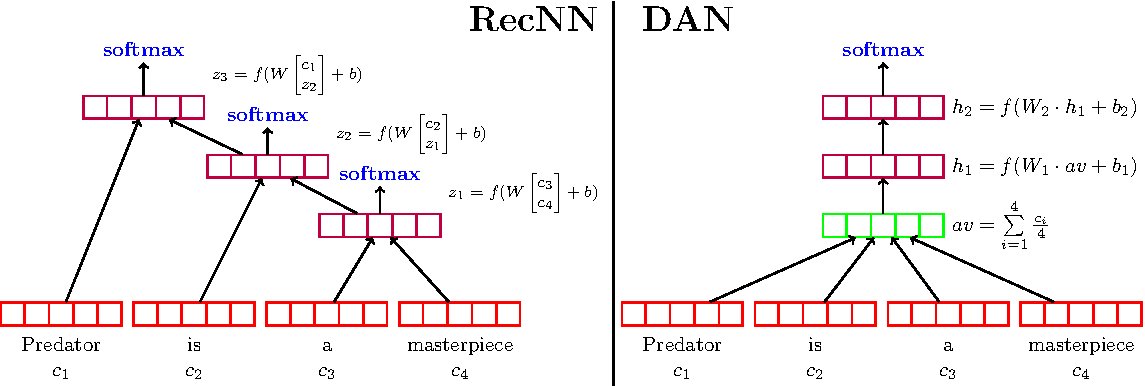
\includegraphics[scale=0.8]{2015_acl_dan/figures/dan_recnn_actualfinal.pdf}
  \caption{On the left, a \recnn\ is given an input sentence for sentiment
          classification. Softmax layers are placed above every internal node to
          avoid vanishing gradient issues. On the right is a two-layer
          \dan\ taking the same input. While the \recnn\ has to compute a
          nonlinear representation (purple vectors) for every node in the parse tree of its
          input, this \dan\ only computes two nonlinear layers for every
          possible input. }
  \label{fig:dan}
\end{figure*}


























Our goal is to marry the speed of unordered functions with the accuracy of
syntactic functions. In this section, we first describe a
class of unordered composition functions dubbed ``neural bag-of-words models''
(\nbow). We then explore more complex syntactic functions designed to avoid many
of the pitfalls associated with \nbow\ models. Finally, we present the deep
averaging network (\dan), which stacks nonlinear layers over the
traditional \nbow\ model and achieves performance on par with or better than
that of syntactic functions.

\subsection{Neural Bag-of-Words Models}\label{sec:nbow}

For simplicity, consider text classification: map an input sequence
of tokens $X$ to one of $k$ labels.  We first apply a composition
function $g$ to the sequence of word embeddings $\boldsymbol{v}_w$ for $w\in X$.
The output of this composition function is a vector $\boldsymbol{z}$ that serves
as input to a logistic regression function.





In our instantiation of \nbow, $g$ averages word embeddings\footnote{Preliminary
  experiments indicate that averaging outperforms the vector sum used in
 \nbow\ from~\newcite{kalchbrenner2014convolutional}.}


\begin{equation}\label{eq:ave}
\boldsymbol{z} = g(w \in X) = \frac 1 {\norm{X}} {\sum_{w \in X} \boldsymbol{v}_w}.
\end{equation}
Feeding $\boldsymbol{z}$ to a softmax layer induces estimated probabilities for each output label
\begin{equation}\label{eq:2}
	\hat y = \mbox{softmax}(\text{\textbf{W}}_s\cdot \boldsymbol{z} + \boldsymbol{b}),
\end{equation}
where the softmax function is
\begin{equation}\label{eq:softmax}
	\mbox{softmax}(\boldsymbol{q}) =  \frac{\exp{\boldsymbol{q}}}{\sum_{j=1}^k \exp{\boldsymbol{q}_j}}
\end{equation}
$\text{\textbf{W}}_s$ is a $k\times d$ matrix for a dataset with $k$ output
labels, and $\boldsymbol{b}$ is a bias term.




We train the \nbow\ model to minimize cross-entropy error, which for a single
training instance with ground-truth label $y$ is
\begin{equation}\label{eq:crossent}
	\ell (\hat y) = \sum\limits_{p=1}^k y_p\log(\hat y_p).
\end{equation}

Before we describe our deep extension of the \nbow\ model, we take a quick
detour to discuss syntactic composition functions.  Connections to other
representation frameworks are discussed further in Section~\ref{sec:experiments}.

\subsection{Considering Syntax for Composition}\label{sec:syntax}








Given a sentence like ``You'll be more entertained getting
hit by a bus'', an unordered model like \nbow\ might be deceived by the word ``entertained''
to return a positive prediction.  In contrast, syntactic composition functions
rely on the order and structure of the input to learn how one word or phrase
affects another, sacrificing computational efficiency in the process. In subsequent sections, we argue that this complexity is not matched by a corresponding gain in
performance.





Recursive neural networks (\recnn s) are syntactic functions that rely on natural language's inherent structure to achieve state-of-the-art accuracies on sentiment analysis tasks~\cite{taiacl15}. As in \nbow{}, each word type has an associated embedding. However, the composition function $g$ now depends on a \emph{parse tree} of the input sequence. The representation for any internal node in a binary parse tree is computed as a nonlinear function of the representations of its children (Figure~\ref{fig:dan}, left). A more powerful \recnn\ variant is the recursive neural tensor network (\rntn), which modifies $g$ to include a costly tensor product~\cite{socher2013recursive}.
















While \recnn s can model complex linguistic phenomena like
negation~\cite{Hermann:2013:CVSC}, they require much more training time than
\nbow\ models.  The nonlinearities and matrix/tensor products at each node of
the parse tree are expensive, especially as model dimensionality
increases. \recnn s also require an error signal at \emph{every} node.  One root
softmax is not strong enough for the model to learn compositional relations and leads to worse accuracies than standard bag-of-words models~\cite{jiweirnn}.
Finally, \recnn s require relatively consistent syntax between
training and test data due to their reliance on parse trees and thus cannot
effectively incorporate out-of-domain data, as we show in our question-answering
experiments. \newcite{kim:2014:EMNLP2014} shows that some of these issues can be avoided by using a convolutional network instead of a \recnn, but the computational complexity increases even further (see Section~\ref{sec:experiments} for runtime comparisons).

What contributes most to the power of syntactic functions: the compositionality
or the nonlinearities? \newcite{socher2013recursive} report that
removing the nonlinearities from their \recnn\ models drops performance on the
Stanford Sentiment Treebank by over 5\% absolute accuracy. Most unordered functions are linear
mappings between bag-of-words features and output labels, so might they suffer
from the same issue? To isolate the effects of syntactic composition from the
nonlinear transformations that are crucial to \recnn\ performance, we
investigate how well a deep version of the \nbow\ model performs on tasks that
have recently been dominated by syntactically-aware models.

\section{Deep Averaging Networks}\label{sec:dan}






The intuition behind deep feed-forward neural networks is that each layer learns
a more abstract representation of the input than the previous
one~\cite{bengio2013representation}. We can apply this concept to the
\nbow\ model discussed in Section~\ref{sec:nbow} with the expectation that each
layer will increasingly magnify small but meaningful differences in the word
embedding average. To be more concrete, take $s_1$ as the sentence ``I really
loved Rosamund Pike's performance in the movie Gone Girl'' and generate $s_2$
and $s_3$ by replacing ``loved'' with ``liked'' and then again by
``despised''. The vector averages of these three sentences are almost
identical, but the averages associated with the synonymous sentences $s_1$ and
$s_2$ are slightly more similar to each other than they are to $s_3$'s average.







Could adding depth to \nbow\ make small such distinctions 
as this one more apparent? In Equation~\ref{eq:ave}, we compute
$\boldsymbol{z}$, the vector representation for input text $X$, by
averaging the word vectors $\boldsymbol{v}_{w \in X}$. Instead of
directly passing this representation to an output layer, we can
further transform $\boldsymbol{z}$ by adding more layers before
applying the softmax. Suppose we have $n$ layers,
$\boldsymbol{z}_{1\dots n}$. We compute each layer 
\begin{equation}
\label{eq:dan}
	\boldsymbol{z}_i = g(\boldsymbol{z}_{i - 1}) = f(\text{\textbf{W}}_i\cdot \boldsymbol{z}_{i - 1} + \boldsymbol{b}_i)
\end{equation}
and feed the final layer's representation, $\boldsymbol{z}_n$, to a softmax
layer for prediction (Figure~\ref{fig:dan}, right).

This model, which we call a deep averaging network (\dan), is still unordered,
but its depth allows it to capture subtle variations in the input better than
the standard \nbow\ model. Furthermore, computing each layer requires just a
single matrix multiplication, so the complexity scales with the number of layers
rather than the number of nodes in a parse tree. In practice, we find no
significant difference between the training time of a \dan\ and that of the
shallow \nbow\ model.

\subsection{Word Dropout Improves Robustness}




Dropout regularizes neural networks by randomly setting hidden and/or input
units to zero with some probability
$p$~\cite{hintondropout,srivastava2014dropout}. Given a neural network with $n$
units, dropout prevents overfitting by creating an ensemble of $2^n$ different
networks that share parameters, where each network consists of some combination
of dropped and undropped units. Instead of dropping units,
a natural extension for the \dan\ model is to randomly drop word tokens' entire
\emph{word embeddings} from the vector average. Using this method, which we call
\emph{word dropout}, our network theoretically sees $2^{|X|}$ different token sequences for each
input $X$.

We posit a vector $\boldsymbol{r}$ with $|X|$ independent Bernoulli trials, each
of which equals 1 with probability $p$. The embedding $\boldsymbol{v}_w$ for
token $w$ in $X$ is dropped from the average if $\boldsymbol{r}_w$ is 0, which
exponentially increases the number of unique examples the network sees during
training.  This allows us to modify Equation~\ref{eq:ave}:
\begin{align}\label{eq:dropped}
&\boldsymbol{r}_w \sim \text{Bernoulli}(p) \\
&\hat X = \{w | w \in X \text{ and } \boldsymbol{r}_w > 0\} \\
& \boldsymbol{z} = g(w \in X) = \frac{\sum_{w \in \hat X} \boldsymbol{v}_w}{\norm{\hat X}}.
\end{align}

Depending on the choice of $p$, many of the ``dropped'' versions of an original
training instance will be very similar to each other, but for shorter inputs
this is less likely. We might drop a very important token, such as ``horrible''
in ``the crab rangoon was especially horrible''; however, since the number of
word types that are predictive of the output labels is low compared to
non-predictive ones (e.g., neutral words in sentiment analysis), we always see
improvements using this technique.

Theoretically, word dropout can also be applied to other neural
network-based approaches. However, we observe no significant
performance differences in preliminary experiments when applying word
dropout to leaf nodes in \recnn s for sentiment analysis (dropped leaf
representations are set to zero vectors), and it slightly hurts
performance on the question answering task. 



























\section{Experiments}
\label{sec:experiments}


\begin{table}
\footnotesize
\begin{tabular}{cccccc}
\toprule
Model & RT & SST & SST & IMDB & Time \\
& & fine & bin & & (s)\\
\midrule
\footnotesize DAN-ROOT & --- & 46.9 & 85.7 & --- & \bf 31\\
\footnotesize DAN-RAND & 77.3 & 45.4 & 83.2 & 88.8 & 136\\
\footnotesize DAN & 80.3 & 47.7 & 86.3 & 89.4 & 136\\
\midrule
\footnotesize NBOW-RAND & 76.2 & 42.3 & 81.4 & 88.9 & 91 \\
\footnotesize NBOW & 79.0 & 43.6 & 83.6 & 89.0 & 91 \\
\footnotesize BiNB & --- & 41.9 & 83.1 & --- & ---\\
\footnotesize NBSVM-bi & 79.4 & --- & --- & 91.2 & ---\\
\midrule
\footnotesize RecNN$^*$ & 77.7 & 43.2 & 82.4 & --- & --- \\
\footnotesize RecNTN$^*$ & --- & 45.7 & 85.4 & --- & --- \\
\footnotesize DRecNN & --- & 49.8 & 86.6 & --- & 431\\
\footnotesize TreeLSTM & --- & \bf 50.6 & 86.9 & --- & --- \\
\footnotesize DCNN$^*$ & --- & 48.5 & 86.9 & 89.4 & ---\\
\footnotesize PVEC$^*$ & --- & 48.7 & 87.8 & \bf 92.6 & --- \\
\footnotesize CNN-MC & \bf 81.1 & 47.4 & \bf 88.1 & --- & 2,452 \\
\footnotesize WRRBM$^*$ & --- & --- & --- & 89.2 & ---\\
\bottomrule
\end{tabular}
\caption{\dan s achieve comparable sentiment accuracies to syntactic functions (bottom third of table) but require much less training time (measured as time of a single epoch on the \abr{sst} fine-grained task). Asterisked models are initialized either with different pretrained embeddings or randomly.}

\label{table:sentiment}
\end{table}

We compare \dan s to both the shallow \nbow\ model as well as more complicated
syntactic models on sentence and document-level sentiment analysis and factoid
question answering tasks. The \dan\ architecture we use for each task is almost
identical, differing across tasks only in the type of output layer and the
choice of activation function. Our results show that \dan s outperform other
bag-of-words models and many syntactic models with very little training
time.\footnote{Code at \url{http://github.com/miyyer/dan}.} On the
question-answering task, \dan s effectively
train on out-of-domain data, while \recnn s struggle to reconcile the syntactic
differences between the training and test data.

\subsection{Sentiment Analysis}\label{sec:sst}

Recently, syntactic composition functions have revolutionized both fine-grained
and binary (positive or negative) sentiment analysis. We conduct sentence-level
sentiment experiments on the Rotten Tomatoes (\abr{rt}) movie reviews
dataset~\cite{pang2005seeing} and its extension with phrase-level labels, the
Stanford Sentiment Treebank (\abr{sst}) introduced
by~\newcite{socher2013recursive}. Our model is also effective on the
document-level \abr{imdb} movie review dataset of~\newcite{maas2011}.

\subsubsection{Neural Baselines}

Most neural approaches to sentiment analysis are variants of either recursive or
convolutional networks. Our recursive neural network baselines include standard
\recnn s~\cite{SocherEtAl2011:RAE}, \rntn s, the deep recursive network
(\drnn) proposed by~\newcite{irsoy-drsv}, and the \tlstm\ of~\cite{taiacl15}. Convolutional network baselines
include the dynamic convolutional
network~\cite[\dcnn]{kalchbrenner2014convolutional} and the convolutional neural
network multi-channel~\cite[\cnnmc]{kim:2014:EMNLP2014}. Our other neural
baselines are the sliding-window based paragraph
vector~\cite[\pvec]{le2014distributed}\footnote{\pvec\ is computationally
  expensive at both training and test time and requires enough memory to store a
  vector for every paragraph in the training data.} and the word-representation
restricted Boltzmann machine~\cite[\wrrbm]{dahl2012training}, which only works
on the document-level~\abr{imdb} task.\footnote{The~\wrrbm\ is trained using a
  slow Metropolis-Hastings algorithm.}

\subsubsection{Non-Neural Baselines}

We also compare to non-neural baselines, specifically the bigram na\"ive Bayes
(\binb) and na\"ive Bayes support vector machine (\nbsvm) models introduced by
\newcite{sidaw12simple}, both of which are memory-intensive due to huge feature
spaces of size $|V|^2$.

\subsubsection{DAN Configurations}

In Table~\ref{table:sentiment}, we compare a variety of \dan\ and
\nbow\ configurations\footnote{Best hyperparameters chosen by cross-validation:
  three 300-d ReLu layers, word dropout probability $p=0.3$, L2 regularization
  weight of 1e-5 applied to all parameters} to the baselines described above. In
particular, we are interested in not only comparing \dan\ accuracies to those of
the baselines, but also how initializing with pretrained embeddings and
restricting the model to only root-level labels affects performance. With this
in mind, the \nbowr\ and \danr\ models are initialized with random
300-dimensional word embeddings, while the other models are initialized with
publicly-available 300-d \texttt{GloVe} vectors trained over the Common
Crawl~\cite{glove2014}.  The \danroot\ model only has access to sentence-level
labels for \abr{sst} experiments, while all other models are trained on labeled
phrases (if they exist) in addition to sentences. We train all \nbow\ and
\dan\ models using AdaGrad~\cite{duchi2011adaptive}.

We apply \dan s to documents by averaging the embeddings for all of a document's
tokens and then feeding that average through multiple layers as before. Since
the representations computed by \dan s are always $d$-dimensional vectors
regardless of the input size, they are efficient with respect to both memory and
computational cost. We find that the hyperparameters selected on the \abr{sst}
also work well for the \abr{imdb} task.

\subsubsection{Dataset Details}

We evaluate over both fine-grained and binary sentence-level classification
tasks on the \abr{sst}, and just the binary task on \abr{rt} and \abr{imdb}. In
the fine-grained \abr{sst} setting, each sentence has a label from zero to five
where two is the neutral class. For the binary task, we ignore all neutral
sentences.\footnote{Our fine-grained \abr{sst} split is \{train: 8,544, dev:
  1,101, test: 2,210\}, while our binary split is \{train: 6,920, dev:872,
  test:1,821\}. Split sizes increase by an order of magnitude when labeled
  phrases are added to the training set. For \abr{rt}, we do 10-fold CV over a
  balanced binary dataset of 10,662 sentences. Similarly, for the \abr{imdb}
  experiments we use the provided balanced binary training set of 25,000
  documents.}

\subsubsection{Results}

The \dan\ achieves the second best reported result on the \abr{rt} dataset,
behind only the significantly slower \cnnmc\ model. It's also competitive with more complex models on the \abr{sst} and outperforms
 the \dcnn\ and \wrrbm\ on the document-level \abr{imdb}
task. Interestingly, the \dan\ achieves good performance on the \abr{sst} when
trained with only sentence-level labels, indicating that it does not suffer from
the vanishing error signal problem that plagues \recnn s. Since acquiring
labelled phrases is often expensive~\cite{sayeed-12,IyyerEtAl2014}, this result
is promising for large or messy datasets where fine-grained annotation is
infeasible.

\subsubsection{Timing Experiments}

\dan s require less time per epoch and---in general---require fewer epochs than
their syntactic counterparts. We compare \dan\ runtime on the \abr{sst} to
publicly-available implementations of syntactic baselines in the last column of
Table~\ref{table:sentiment}; the reported times are for a single epoch to
control for hyperparameter choices such as learning rate, and all models use
300-$d$ word vectors. Training a \dan\ on just sentence-level labels on the
\abr{sst} takes under five minutes on a single core of a laptop; when labeled
phrases are added as separate training instances, training time jumps to twenty
minutes.\footnote{We also find that \dan s take significantly fewer epochs to
  reach convergence than syntactic models.} All timing experiments were performed on a
single core of an Intel I7 processor with 8GB of RAM.



\subsection{Factoid Question Answering}


\begin{table}[t]
\begin{center}
\begin{tabular}{lrrrr}
\toprule
Model    & Pos 1 & Pos 2 & Full & \footnotesize Time(s) \\
\midrule
BoW-DT & 35.4 & 57.7 & 60.2 & --- \\
IR & 37.5 & 65.9 & 71.4 & N/A \\
QANTA & 47.1 & 72.1 & 73.7 & 314 \\
DAN & 46.4 & 70.8 & 71.8 & \bf 18 \\
\midrule
IR-WIKI & 53.7 & \bf 76.6 & \bf 77.5 & N/A\\
QANTA-WIKI & 46.5 & 72.8 & 73.9 & 1,648 \\
DAN-WIKI & \bf 54.8 & 75.5 & 77.1 & 119 \\
\bottomrule
\end{tabular}

\end{center}
\caption{The \dan\ achieves slightly lower accuracies than the more complex \qanta\ in much less training time, even at
  early sentence positions where compositionality plays a bigger role. When Wikipedia is added to the training set (bottom half of table), the \dan\ outperforms \qanta\ and achieves comparable accuracy to a state-of-the-art information retrieval baseline, which highlights a benefit of ignoring word order for this task.}
\label{table:qb}
\end{table}

\begin{figure}	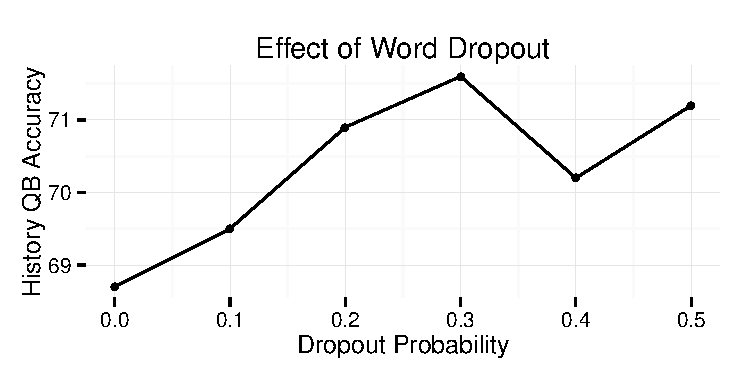
\includegraphics[scale=0.6]{2015_acl_dan/figures/dropout_effect.pdf}
	\caption{Randomly dropping out 30\% of words from the vector average is
          optimal for the quiz bowl task, yielding a gain in absolute accuracy
          of almost 3\% on the quiz bowl question dataset compared to the same model trained with no word dropout.}
\label{fig:sdrop}

\end{figure}

\dan s work well for sentiment analysis, but how do they do on other \abr{nlp}
tasks?  We shift gears to a paragraph-length factoid question answering task and
find that our model outperforms other unordered functions as well as a more
complex syntactic \recnn\ model. More interestingly, we find that unlike the
\recnn, the \dan\ significantly benefits from out-of-domain Wikipedia training
data.



Quiz bowl is a trivia competition in which players are asked
four-to-six sentence questions about entities (e.g., authors, battles,
or events). It is an ideal task to evaluate \dan s because there is
prior work using both syntactic and unordered models for quiz bowl
question answering. In \newcite{Boyd-Graber:Satinoff:He:III-2012},
na\"{\i}ve Bayes bag-of-words models ({\bf \textsc{bow-dt}}) and sequential language models
work well on easy questions but poorly on harder ones. A
dependency-tree \recnn\ called \qanta\ proposed
in~\newcite{IyyerQA2014} shows substantial improvements, leading to
the hypothesis that correctly modeling compositionality is crucial for answering
hard questions.

\subsubsection{Dataset and Experimental Setup}

To test this, we train a \dan\ over the history questions from
\newcite{IyyerQA2014}.\footnote{The training set contains 14,219 sentences over
  3,761 questions. For more detail about data and baseline systems,
  see~\newcite{IyyerQA2014}.} This dataset is augmented with 49,581
sentence/page-title pairs from the Wikipedia articles associated with the
answers in the dataset. For fair comparison with \qanta, we use a normalized
tanh activation function at the last layer instead of ReLu, and we also change
the output layer from a softmax to the margin ranking
loss~\cite{weston2011wsabie} used in \qanta. We initialize the \dan\ with the same pretrained 100-d word embeddings that were used to initialize \qanta.

We also evaluate the effectiveness of word dropout on this task in
Figure~\ref{fig:sdrop}. Cross-validation indicates that $p=0.3$ works best for question answering, although the improvement in
accuracy is negligible for sentiment analysis. Finally, continuing the trend observed in
the sentiment experiments, \dan\ converges much faster than \qanta.

\subsubsection{DANs Improve with Noisy Data}

Table~\ref{table:qb} shows that while \dan\ is slightly worse than \qanta\
when trained only on question-answer pairs, it improves when trained on
additional out-of-domain Wikipedia data (\danw), reaching performance comparable
to that of a state-of-the-art information retrieval system (\irw). \qanta, in
contrast, barely improves when Wikipedia data is added (\qantaw) possibly due to
the syntactic differences between Wikipedia text and quiz bowl question text.

The most common syntactic structures in quiz bowl sentences are imperative
constructions such as ``Identify this British author who wrote Wuthering
Heights'', which are almost never seen in Wikipedia. Furthermore, the subject of
most quiz bowl sentences is a pronoun or pronomial mention referring to the
answer, a property that is not true of Wikipedia sentences (e.g., ``Little of
Emily's work from this period survives, except for poems spoken by
characters.''). Finally, many Wikipedia sentences do not uniquely identify the
title of the page they come from, such as the following sentence from Emily
Bront{\"e}'s page: ``She does not seem to have made any friends outside her
family.'' While noisy data affect both \dan\ and \qanta, the latter is
further hampered by the syntactic divergence between quiz bowl questions and
Wikipedia, which may explain the lack of improvement in accuracy.




\section{How Do DANs Work?}
\label{sec:discussion}

In this section we first examine how the deep layers of the \dan\ amplify tiny
differences in the vector average that are predictive of the output
labels. Next, we compare \dan s to \drnn s on sentences that contain negations
and contrastive conjunctions and find that both models make similar errors
despite the latter's increased complexity. Finally, we analyze the predictive
ability of unsupervised word embeddings on a simple sentiment task in an effort
to explain why initialization with these embeddings improves the \dan.




\begin{figure}[t!]
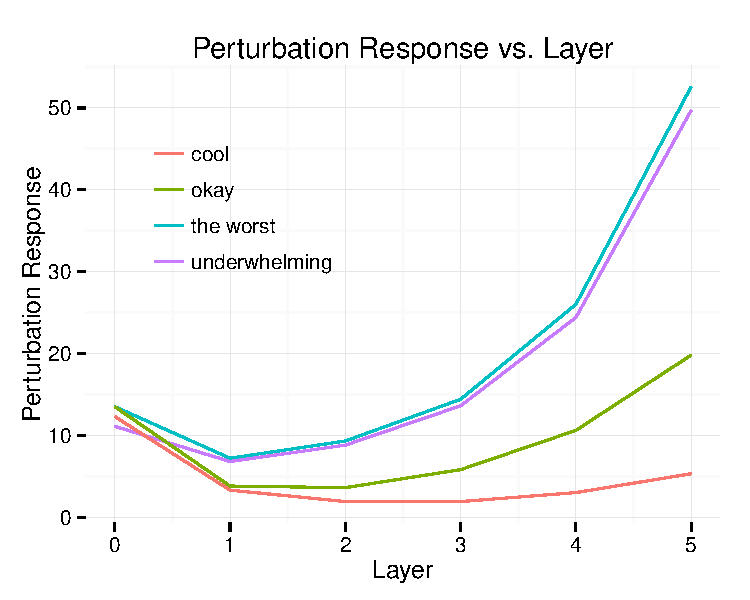
\includegraphics[scale=0.6]{2015_acl_dan/figures/perturb_2.pdf}
  \caption{Perturbation response (difference in 1-norm) at each layer of a 5-layer \dan\ after replacing \emph{awesome} in \emph{the film's performances were awesome} with four words of varying sentiment polarity. While the shallow \nbow\ model does not show any meaningful distinctions, we see that as the network gets deeper, negative sentences are increasingly different from the original positive sentence.}
\label{fig:perturb}

\end{figure}

\begin{figure}[t!]
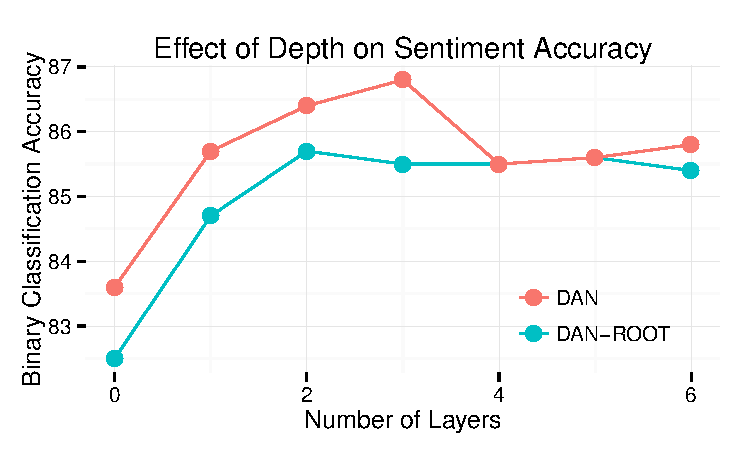
\includegraphics[scale=0.6]{2015_acl_dan/figures/layers.pdf}
  \caption{Two to three layers is optimal for the \dan\ on the \abr{sst} binary sentiment
          analysis task, but adding any depth at all is an improvement over the
          shallow \nbow\ model.}
\label{fig:slayers}
\end{figure}









\subsection{Perturbation Analysis}

Following the work of \newcite{irsoy-drsv}, we examine our network by measuring
the response at each hidden layer to perturbations in an input sentence. In
particular, we use the template \emph{the film's performances were awesome} and
replace the final word with increasingly negative polarity words (\emph{cool},
\emph{okay}, \emph{underwhelming}, \emph{the worst}). For each perturbed
sentence, we observe how much the hidden layers differ from those associated
with the original template in 1-norm.

Figure~\ref{fig:perturb} shows that as a \dan\ gets deeper, the differences
between negative and positive sentences become increasingly amplified. While
nonexistent in the shallow \nbow\ model, these differences are visible even with
just a single hidden layer, thus explaining why deepening the \nbow\ improves
sentiment analysis as shown in Figure~\ref{fig:slayers}.

\begin{table*}[ht]
  \begin{center}
    \begin{tabular}{p{8cm}ccc}
    \toprule
    Sentence & \dan & \drnn & Ground Truth \\
    \midrule
  \footnotesize
    a \hemph{lousy}  movie that's \hemph{not} merely \hemph{unwatchable}, but also \hemph{unlistenable} & \hemph{negative} & \hemph{negative} & \hemph{negative}\\
    \footnotesize
  if you're \hemph{not} a \kemph{prepubescent} \eemph{girl}, you'll be \aemph{laughing} at \hemph{britney} \hemph{spears}' \eemph{movie-starring} \eemph{debut} whenever it does \hemph{n't} have you \kemph{impatiently} \hemph{squinting} at your \eemph{watch} & \kemph{negative} & \kemph{negative} & \kemph{negative} \\
    \footnotesize
  \aemph{blessed} with \aemph{immense} \aemph{physical} \aemph{prowess} he \kemph{may} well be, but \hemph{ahola} is \eemph{simply} \hemph{not} an \eemph{actor} & \eemph{positive} & neutral & \kemph{negative}\\
    \footnotesize
  who \aemph{knows} what \kemph{exactly} \kemph{godard} is on about in this \eemph{film}, but his \aemph{words} and images do \hemph{n't} have to \aemph{add} up to \aemph{mesmerize} you. & \eemph{positive} & \eemph{positive} & \eemph{positive}\\
    \footnotesize
  it's so \aemph{good} that its \kemph{relentless}, \aemph{polished} \eemph{wit} can \eemph{withstand} \hemph{not} \kemph{only} \hemph{inept} school \aemph{productions}, but even \aemph{oliver} \aemph{parker}'s movie \eemph{adaptation} & \kemph{negative} & \eemph{positive} & \eemph{positive}\\
    \footnotesize
  \kemph{too} \hemph{bad}, but \aemph{thanks} to some \aemph{lovely} \aemph{comedic} \eemph{moments} and several \aemph{fine} \eemph{performances}, it's \hemph{not} a \hemph{total} \hemph{loss} & \kemph{negative} & \kemph{negative} & \eemph{positive}\\
  \midrule
    \footnotesize
  this movie was \hemph{not} \aemph{good} & \kemph{negative} & \kemph{negative} & negative\\
    \footnotesize
  this movie was \aemph{good} & \aemph{positive} & \aemph{positive} & positive\\
    \footnotesize
  this movie was \hemph{bad} & \hemph{negative} & \kemph{negative} & negative\\
    \footnotesize
  the movie was \hemph{not} \hemph{bad} & \hemph{negative} & \kemph{negative} & positive\\
    \bottomrule
    \end{tabular}
    \end{center}
  \caption{Predictions of \dan\ and \drnn\ models on real (top) and synthetic
    (bottom) sentences that contain negations and contrastive conjunctions. In
    the first column, words colored red individually predict the negative label
    when fed to a \dan, while blue words predict positive. The \dan\ learns that
    the negators \emph{not} and \emph{n't} are strong negative predictors, which
    means it is unable to capture double negation as in the last real example
    and the last synthetic example. The \drnn\ does slightly better on the synthetic
    double negation, predicting a lower negative polarity.}

\label{table:examples}
\end{table*}


\subsection{Handling Negations and ``but'': Where Syntax is Still Needed }

While \dan s outperform other bag-of-words models, how can they model linguistic
phenomena such as negation without considering word order? To evaluate \dan s
over tougher inputs, we collect 92 sentences, each of which contains at least one
negation and one contrastive conjunction, from the dev and test sets of the
\abr{sst}.\footnote{We search for non-neutral sentences containing \emph{not} /
  \emph{n't}, and \emph{but}. 48 of the sentences are positive while 44 are
  negative.} Our fine-grained accuracy is \emph{higher} on this subset than on
the full dataset, improving almost five percent absolute accuracy to
53.3\%. The \drnn\ model of \newcite{irsoy-drsv} obtains a similar
accuracy of 51.1\%, contrary to our intuition that syntactic functions should
outperform unordered functions on sentences that clearly require syntax to
understand.\footnote{Both models are initialized with pretrained 300-d GloVe embeddings for fair comparison.}

Are these sentences truly difficult to classify? A close inspection reveals that
both the \dan\ and the \drnn\ have an overwhelming tendency to predict negative
sentiment (60.9\% and 55.4\% of the time for the \dan\ and \drnn\ respectively) when they see a negation compared
to positive sentiment (35.9\% for \dan s, 34.8\% for \drnn s). If we further
restrict our subset of sentences to only those with positive ground truth
labels, we find that while both models struggle, the \drnn\ obtains 41.7\% accuracy, outperforming the \dan's 37.5\%.

To understand why a negation or contrastive conjunction triggers a negative
sentiment prediction, we show six sentences from the negation subset and four
synthetic sentences in Table~\ref{table:examples}, along with both models'
predictions. The token-level predictions in the table (shown as colored boxes)
are computed by passing each token through the \dan\ as separate test
instances.  The tokens \emph{not} and \emph{n't} are strongly predictive of
negative sentiment. While this simplified ``negation'' works for many
sentences in the datasets we consider, it prevents the \dan\ from reasoning
about double negatives, as in ``this movie was not bad''. The \drnn\ does
slightly better in this case by predicting a lesser negative polarity than the
\dan; however, we theorize that still more powerful syntactic composition
functions (and more labelled instances of negation and related phenomena) are
necessary to truly solve this problem.

























\subsection{Unsupervised Embeddings Capture Sentiment}

Our model consistently converges slower to a worse solution (dropping 3\% in
absolute accuracy on coarse-grained \abr{sst}) when we randomly initialize the
word embeddings. This does not apply to just \dan s; both convolutional and
recursive networks do the same~\cite{kim:2014:EMNLP2014,irsoy-drsv}. Why are
initializations with these embeddings so crucial to obtaining good performance?
Is it possible that unsupervised training algorithms are already capturing
sentiment?

We investigate this theory by conducting a simple experiment: given a sentiment
lexicon containing both positive and negative words, we train a logistic
regression to discriminate between the associated word embeddings (without any
fine-tuning). We use the lexicon created by~\newcite{hu2004mining}, which
consists of 2,006 positive words and 4,783 negative words. We balance and split
the dataset into 3,000 training words and 1,000 test words. Using
300-dimensional \texttt{GloVe} embeddings pretrained over the Common Crawl, we
obtain over 95\% accuracy on the unseen test set, supporting the hypothesis that
unsupervised pretraining over large corpora can capture properties such as
sentiment.

Intuitively, after the embeddings are fine-tuned during \dan\ training, we might
expect a decrease in the norms of stopwords and an increase in the norms of
sentiment-rich words like ``awesome'' or ``horrible''. However, we find no
significant differences between the $L_2$ norms of stopwords and words in the
sentiment lexicon of~\newcite{hu2004mining}.

\section{Related Work}
\label{sec:related}








Our \dan\ model builds on the successes of both
simple vector operations and neural network-based models for compositionality.

There are a variety of element-wise vector operations that could replace the average used in the \dan.~\newcite{MitchellL08} experiment with many of them to model the compositionality of short phrases. Later, their work was extended to take into account the
syntactic relation between
words~\cite{erk08,baroni2010nouns,kartsaklis2013prior} and
grammars~\cite{coecke2010mathematical,grefenstette2011experimental}. While the average works best for the tasks that we consider,~\newcite{simcompass} find that simply summing \texttt{word2vec} embeddings outperforms all other methods on the SemEval 2014 phrase-to-word and sentence-to-phrase similarity tasks.

Once we compute the embedding average in a \dan, we feed it to a deep neural
network. In contrast, most previous work on neural network-based methods for
\abr{nlp} tasks explicitly model word order. Outside of sentiment analysis, \recnn-based approaches have been
successful for tasks such as parsing~\cite{SocherEtAl2013:CVG}, machine translation~\cite{liu2014recursive}, and paraphrase
detection~\cite{SocherEtAl2011:PoolRAE}. Convolutional networks also model word order in
local windows and have achieved performance comparable to or better than that of
\recnn s on many tasks~\cite{collobert2008unified,kim:2014:EMNLP2014}. Meanwhile, feed-forward architectures like that of the \dan\ have been used for language modeling~\cite{Bengio03aneural}, selectional preference acquisition~\cite{van2014neural}, and dependency parsing~\cite{chen2014fast}.












\section{Future Work}
\label{sec:future}
In Section~\ref{sec:discussion}, we showed that the performance of our \dan\ model
worsens on sentences that contain lingustic phenomena such as double
negation. One promising future direction is to cascade classifiers such that syntactic models are used only when a \dan\ is not confident
in its prediction. We can also extend the \dan 's success at incorporating out-of-domain training data to sentiment analysis: imagine training a \dan\ on labeled tweets for classification on newspaper reviews. Another potentially interesting application is to add gated units to a \dan,as has been done for recurrent and recursive neural networks~\cite{hochreiter1997long,cho2014learning,sutskever2014sequence,taiacl15}, to drop useless words rather than randomly-selected ones.




\section{Conclusion}
\label{sec:conclusion}
In this paper, we introduce the deep averaging network, which feeds an unweighted average of word vectors through multiple hidden layers before classification. The \dan\ performs competitively with more complicated neural networks that explicitly model semantic and syntactic compositionality. It is further strengthened by word dropout, a regularizer that reduces input redundancy. \dan s obtain close to state-of-the-art accuracy on both sentence and document-level sentiment analysis and factoid question-answering tasks with much less training time than competing methods; in fact, all experiments were performed in a matter of minutes on a single laptop core. We find that both \dan s and syntactic functions make similar errors given syntactically-complex input, which motivates research into more powerful models of compositionality.
\section*{Acknowledgments}
We thank Ozan \.Irsoy not only for many insightful discussions but
also for suggesting some of the experiments that we included in the
paper. We also thank the anonymous reviewers, Richard Socher, Arafat
Sultan, and the members of the UMD ``Thinking on Your Feet'' research
group for their helpful comments. This work was supported by \abr{nsf}
Grant IIS-1320538.  Boyd-Graber is also supported by \abr{nsf} Grants
\abr{ccf}-1409287 and \abr{ncse}-1422492.  Any opinions, findings,
conclusions, or recommendations expressed here are those of the
authors and do not necessarily reflect the view of the sponsor.


\clearpage

\bibliographystyle{style/acl2015}
\footnotesize
\bibliography{bib/journal-full,bib/miyyer,bib/jbg}

\end{document}
